% set table width
\newcommand{\PreserveBackslash}[1]{\let\temp=\\#1\let\\=\temp}
\newcolumntype{C}[1]{>{\PreserveBackslash\centering}p{#1}}
% used for heatmap
\newcommand*{\MinNumber}{0}%
\newcommand*{\MaxNumber}{1}%
\newcommand{\ApplyGradient}[1]{%
	\pgfmathsetmacro{\PercentColor}{100.0*(#1-\MinNumber)/(\MaxNumber-\MinNumber)}
	\hspace{-0.33em}\colorbox{white!\PercentColor!myblack}{}
}
\newcolumntype{Q}{>{\collectcell\ApplyGradient}c<{\endcollectcell}}

	\begin{center}
		\renewcommand{\arraystretch}{0}
		\setlength{\tabcolsep}{5mm}
		\setlength{\fboxsep}{2.2mm} % box size
		\begin{tabular}{C{.40\textwidth}C{.40\textwidth}C{.40\textwidth}C{.40\textwidth}}
			\setlength{\tabcolsep}{0pt}
			\subfigure [\small{自注意力}] {
				\begin{tabular}{ccC{1em}}
					\setlength{\tabcolsep}{0pt}
					~
					&
					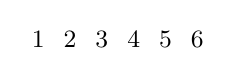
\begin{tikzpicture}
					\begin{scope}			
					\node [inner sep=1.5pt] (w1) at (0,0) {\small{$1$} };
					
					\foreach \x/\y/\z in {2/1/$2$, 3/2/$3$, 4/3/$4$, 5/4/$5$, 6/5/$6$}
					{
						\node [inner sep=1.5pt,anchor=south west] (w\x) at ([xshift=1.15em]w\y.south west) {\small{\z} };
					}
					\end{scope}
					\end{tikzpicture}
					\\
					\renewcommand\arraystretch{1}
					\begin{tabular}{c}
						\setlength{\tabcolsep}{0pt}
						\small{$1\ \ $} \\
						\small{$2\ $} \\
						\small{$3\ $} \\
						\small{$4\ $} \\
						\small{$5\ $} \\
						\small{$6\ $} \\
					\end{tabular}
					&
					%\setlength{\tabcolsep}{0pt}
					\begin{tabular}{*{6}{Q}}
						0.0000 & 0.5429 & 0.5138 & 0.4650 & 0.5005 & 0.5531 \\

                        0.5429 & 0.0000 & 0.0606 & 0.0630 & 0.0703 & 0.0332 \\

                        0.5138 & 0.0606 & 0.0000 & 0.0671 & 0.0472 & 0.0296 \\

                        0.4650 & 0.0630 & 0.0671 & 0.0000 & 0.0176 & 0.0552 \\

                        0.5005 & 0.0703 & 0.0472 & 0.0176 & 0.0000 & 0.0389 \\

                        0.5531 & 0.0332 & 0.0296 & 0.0552 & 0.0389 & 0.0000 \\
					\end{tabular}
&
				\end{tabular}
			}
			&
			
			\subfigure [\small{编码-解码注意力}] {
				\setlength{\tabcolsep}{0pt}
				\begin{tabular}{ccC{1em}}
					\setlength{\tabcolsep}{0pt}
					~
					&
					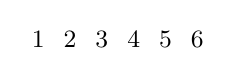
\begin{tikzpicture}
					\begin{scope}
						
					\node [inner sep=1.5pt] (w1) at (0,0) {\small{$1$} };
					\foreach \x/\y/\z in {2/1/$2$, 3/2/$3$, 4/3/$4$, 5/4/$5$, 6/5/$6$}
					{
						\node [inner sep=1.5pt,anchor=south west] (w\x) at ([xshift=1.15em]w\y.south west) {\small{\z} };
					}
					\end{scope}

					\end{tikzpicture}
					\\
					\renewcommand\arraystretch{1}
					\begin{tabular}{c}
						\setlength{\tabcolsep}{0pt}
						\small{$1\ \ $} \\
						\small{$2\ $} \\
						\small{$3\ $} \\
						\small{$4\ $} \\
						\small{$5\ $} \\
						\small{$6\ $} \\
					\end{tabular}
					&
					%\setlength{\tabcolsep}{0pt}
					\begin{tabular}{*{6}{Q}}
                        0.0000 & 0.0175 & 0.2239 & 0.3933 & 0.7986 & 0.3603 \\

                        0.0175 & 0.0000 & 0.1442 & 0.3029 & 0.7295 & 0.3324 \\

                        0.2239 & 0.1442 & 0.0000 & 0.0971 & 0.6270 & 0.4163 \\

                        0.3933 & 0.3029 & 0.0971 & 0.0000 & 0.2385 & 0.2022 \\

                        0.7986 & 0.7295 & 0.6270 & 0.2385 & 0.0000 & 0.0658 \\

                        0.3603 & 0.3324 & 0.4163 & 0.2022 & 0.0658 & 0.0000 \\
					\end{tabular}
&
				\end{tabular}
			}
		\end{tabular}
	\end{center}
